\section{Durchführung}
\subsection{Die Funktionsweise der Wärmepumpe \cite[vgl.][]{man:v206}} % Zitieren soweit notwendig
\label{sec:funktionsweise}

\begin{figure}[H]
    \centering
    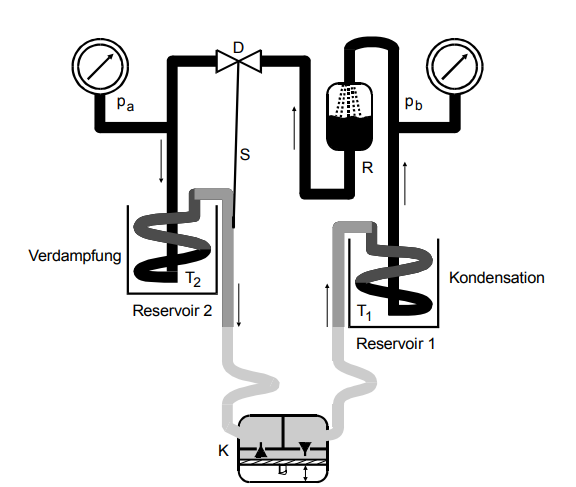
\includegraphics[height=8cm]{prinzipellerAufbau.png}
    \caption[]{Prinzipieller Aufbau einer Wärmepumpe \cite[]{man:v206}.}
    \label{fig:prinzipieller_aufbau}
\end{figure}

Ein prinzipeller Aufbau der Wärmepumpe ist in Abbildung \ref{fig:prinzipieller_aufbau} zu sehen.
Hierbei stehen die Indizes \enquote{1} und \enquote{b} für das warme Reservoir,
während \enquote{2} und \enquote{a} das kalte Reservoir beschreiben.
Die Wärmepumpe pumpt ein Gas in einem abgeschlossenen Kreislauf durch die beiden Reservoirs w und k.
In den Reservoirs besteht der Kreislauf aus Kupferrohren, die zu einer Spirale aufgewickelt sind.
So kann Wärme zwischen den Reservoirs und dem Kreislauf fließen.
Dabei wird durch einen Kompressor K und ein Drosselventil D ein höherer Druck in der Kupferspirale w erzeugt.
Das Gas kondensiert, verliert an Volumen und gibt Wärme an die Umgebung ab.
Die Temperatur in Reservoir w steigt also. 
Das flüssige Gas wird durch das Drosselventil D in den zweiten Teil des Kreislaufes gelassen.
Durch eine technische Vorrichtung R wird sichergestellt, dass nur das flüssige Gas den Kreislauf passiert.
Im zweiten Teil des Kreislaufs wird durch die Pumpe ein Unterdruck im Vergleich zum ersten Teil erzeugt.
Dabei verdampft das Gas wieder, es nimmt an Volumen zu und nimmt Wärme aus der Umgebung auf.
Das Reservoir k wird also kälter.
Eine weitere technische Vorrichtung S gewährleistet, dass das Transportmittel nur im gasförmigen Zustand 
den zweiten Teil des Kreislaufs zur Pumpe hin verlässt.

\subsection{Versuchsdurchführung}
\begin{figure}[H]
    \centering
    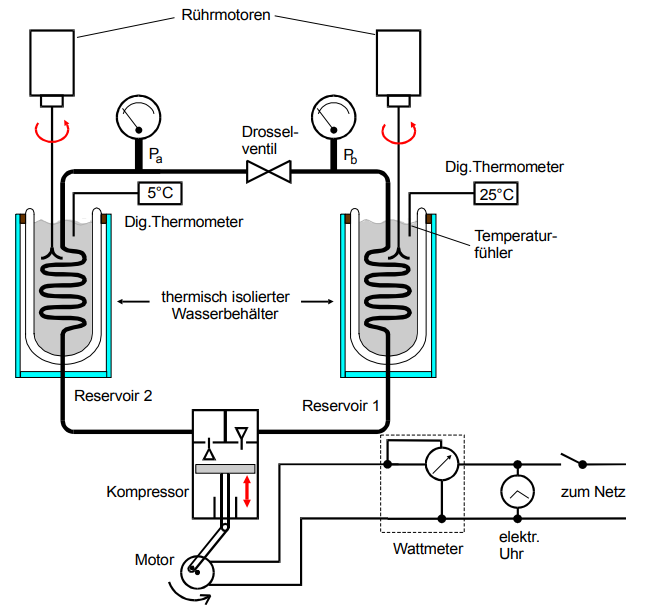
\includegraphics[height = 9cm]{kompletteApparatur.png}
    \caption{Darstellung der kompletten Apparatur \cite[]{man:v206}.}
    \label{fig:kompletteDarstellung}
\end{figure}
\noindent
In Abbildung \ref{fig:kompletteDarstellung} ist eine schematische Dartellung der kompletten Messapparatur zu sehen.
Wie in Abschnitt \ref{sec:funktionsweise} werden auch hier die anderen Indizes verwendet.

\noindent 
Eine Wärmepumpe wie beschrieben wird aufgestellt.
Die beiden Reservoirs werden mit jeweils 3 Litern Wasser befüllt.
Der Druck in beiden Teilen des Gaskreislaufs wird mithilfe von Manometern gemessen.
Im Folgenden steht $p_\text{k}$ für den Druck im kalten Reservoir und $p_\text{w}$ für den Druck im warmen Reservoir.
Dabei werden für $p_\text{k}$ und $p_\text{w}$ zu den eigentlichen Messdaten jeweils $\qty[]{1}{bar}$ hinzu addiert,
was in der Anleitung \cite[]{man:v206} vorgegeben wird und mit dem Versuchsaufbau zu erklären ist. 
Die Temperatur in beiden Reservoirs wird mit digitalen Thermometern gemessen,
wobei $T_\text{k}$ die Temperatur im kalten und $T_\text{w}$ die Temperatur im warmen Reservoir beschreibt.
Die Stromversorgung des Kompressors der Wärmepumpe läuft über ein Wattmeter, um die elektrische Leistung $P$ herauszufinden.
Die Werte bevor die Wärmepumpe angeschaltet wird, werden in der Tabelle \ref{tab:messdaten} bei Minute 0 eingetragen.
Schließlich wird mit dem Handy die Zeit $t$ gestoppt.
Alle 60 Sekunden werden die beiden Temperaturen, die beiden Gasdrücke und die elektrische Leistung abgelesen und notiert.
Hierbei werden die Geräte immer in der gleichen Reihenfolge abgelesen, 
damit die Zeitabstände zwischen den Messungen konsistent bleiben.

